\documentclass[conference]{IEEEtran}
% Some Computer Society conferences also require the compsoc mode option,
% but others use the standard conference format.
%
% If IEEEtran.cls has not been installed into the LaTeX system files,
% manually specify the path to it like:
% \documentclass[conference]{../sty/IEEEtran}
%\usepackage{ifpdf}


\usepackage{cite}
\ifCLASSINFOpdf
  \usepackage[pdftex]{graphicx}
  \usepackage{epstopdf}
\else
  \usepackage[dvips]{graphicx}
\fi

%\usepackage{amsmath}

%\usepackage{algorithmic}

%\usepackage{array}

%\ifCLASSOPTIONcompsoc
%  \usepackage[caption=false,font=normalsize,labelfont=sf,textfont=sf]{subfig}
%\else
%  \usepackage[caption=false,font=footnotesize]{subfig}
%\fi

%\usepackage{fixltx2e}
%\usepackage{stfloats}
%\fnbelowfloat
%\usepackage{dblfloatfix}

%\usepackage{url}



\begin{document}
\title{Image Captioning based on Recurrent Neural Network Model}

% author names and affiliations
% use a multiple column layout for up to three different
% affiliations
\author{\IEEEauthorblockN{Heng Qiao}
\IEEEauthorblockA{Department of Electrical\\ and Computer Engineering\\
University of Florida\\
Email:}
\and
\IEEEauthorblockN{Tong Shao}
\IEEEauthorblockA{Department of Electrical\\ and Computer Engineering\\
University of Florida\\
Email: stlm1991@ufl.edu}
\and
\IEEEauthorblockN{Yichen Liang}
\IEEEauthorblockA{Department of Electrical\\ and Computer Engineering\\
University of Florida\\
Email: }}

% make the title area
\maketitle

% As a general rule, do not put math, special symbols or citations
% in the abstract
\begin{abstract}
Image captioning is the task to automatically describe the content of an image, which is a fundamental problem in artificial intelligence that connects computer vision and natural language processing. In this course project, we plan to develop an image captioning system based on the recurrent neural network(RNN) Model. As the most widely used scheme, two neural networks are introduced. The first one is a pre-trained convolutional neural network (CNN) that converts the image into feature vectors, such as the VggNet, ResNet and Inception. Serving as the core of the scheme, the second one adopts the recurrent neural network (RNN) model. It takes the image feature as the input and generate the word vectors of a sentence (caption). The model is trained to maximize the likelihood of the target description sentence given the training image. Based on this, we aim at implementing some assistant techniques to further improve the performance, such as the semantic structures and more optimized neural network structures. This scheme will be implemented in Tensorflow. Experiments will be conducted on public dataset MS COCO and related evaluation scores such as the BLEU-4 score will be provided. Also, the final report, slides and other related material will be prepared as well.
\end{abstract}

\IEEEpeerreviewmaketitle



\section{Introduction}

Deep learning technology has been widely used in many aspects \cite{krizhevsky2012imagenet}, such as face recognition, natural language processing and etc. It has shown remarkable learning ability in many areas. Among them, the most common form of machine learning, deep or not, is supervised learning \cite{lecun2015deep}. Supervised learning requires labeled training data and typically outputs a label when given a new input \cite{lecun1998gradient}. To deal with inputs with correlations in time such as an sentence, recurrent neural network (RNN) \cite{mikolov2010recurrent}, typically implemented with long short-term memory (LSTM) units, is employed.

Image captioning is the procedure to automatically describe the content of an image, as shown in Fig. \ref{cap_fig}. And there has been a recent surge of interest in developing models that can generate captions for images or videos. Most of these approaches learn a probabilistic model of the caption, conditioned on an image or a video. Most recent work on visual captioning first extracts features from an image, obtaining a fixed-length vector representation of a given image or video. Then a language, usually a recurrent neural network (RNN), typically implemented with long short-term memory (LSTM) units \cite{graves2013speech}, is employed to generate a caption while the image's vector representation is the input \cite{vinyals2015show}.

\begin{figure}
  \centering
  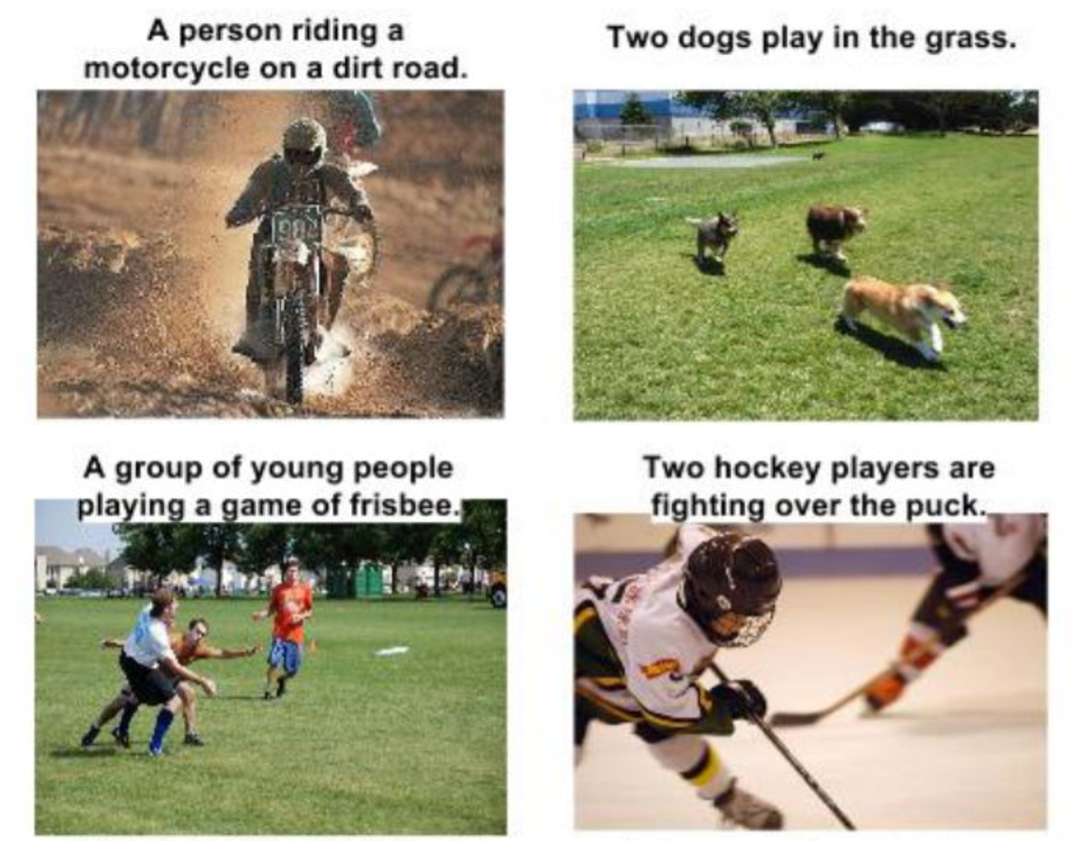
\includegraphics[width=1.0\linewidth]{figures/caption.pdf}
  \caption{Examples of image captioning.}\label{cap_fig}
\end{figure}

Though good results have been achieved, most methods are still far away from human performance and the models usually don't consider the grammar rules. Recent work shows that adding explicit high-level semantic concepts of the input image/video can further improve visual captioning. For instance, in \cite{you2016image}, a model of semantic attention is proposed which selectively attends to semantic concepts through a soft attention mechanism.

goals, deliverables, overview architecture, use cases, modules/subsystems, flowcharts, algorithms, potential results (performance metrics, success evaluation criteria, mock-up result figures x,y,z curves etc.).


\section{Project Description}
We aim at designing a typical image captioning system while adding some techniques to further enhance the performance. The detailed project description is as following.
\subsection{Goals}
Our main goal is to implement an image captioning system which could automatically describe the content of an image as described before. The scheme will be implemented in Tensorflow and experiments will be conducted on MS COCO dataset.

The syetem should be able to produce reasonable captions for input images. And the scores (based on popular metrics) on the MS COCO datasets should be close to, i.e. of the same level as the state-of-the-art methods.

\subsection{Deliverables}

We will implement the scheme in Tensflow. Thus we will provide the codes, the pre-trained model as well as the final report, slides.
\subsection{Overview Architecture}

As shown in Fig. \ref{framework_fig}, the basic architecture has two parts. The first one is a pre-trained convolutional neural network (CNN) that converts the image into feature vectors, such as the VggNet, ResNet and Inception. And the second one adopts the recurrent neural network (RNN) model. It takes the image feature as the input and generate the word vectors of a sentence (caption).

\begin{figure}
  \centering
  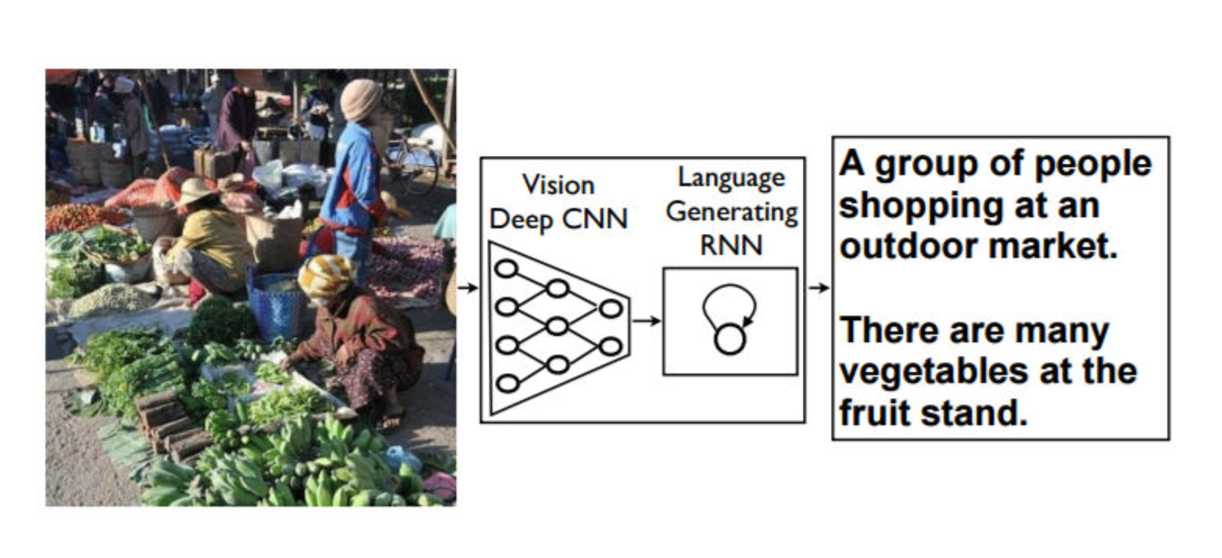
\includegraphics[width=1.0\linewidth]{figures/framework.pdf}
  \caption{Overview Architecture of our image captioning scheme.}\label{framework_fig}
\end{figure}

\subsection{potential results}

As described before, this scheme should produce reasonable captions for input images. We will present some results of images with typical scenes such as sports activities, natural scenes, indoor scenes and etc.
 
Meanwhile, we will test the scheme on the widely used MS COCO dataset. And the scores based on several popular metrics will be provided including the BLEU, METEOR and CIDER. 

We expect our scheme will produce pretty good results on the MS COCO dataset. It should be close to, i.e. of the same level as the state-of-the-art methods such as the Show and Tell \cite{vinyals2015show}.

\subsection{Weekly Progress Plan}
The schedule of each task is as following:
\\1) Scheme design
\\March 4-March 11
\\2) Code implementing
\\March 12-March 31
\\3) Final Report Writing
\\April 1-April 15
\\4) Slides and Presentation
\\April 16-April 23
\bibliographystyle{IEEEtran}
\bibliography{refs}


% that's all folks
\end{document}


